\documentclass{standalone}

%% tikz packages
\usepackage{tikz}
\usetikzlibrary{trees}
\usetikzlibrary{backgrounds}
\usepackage{tikz-dependency}

\begin{document}

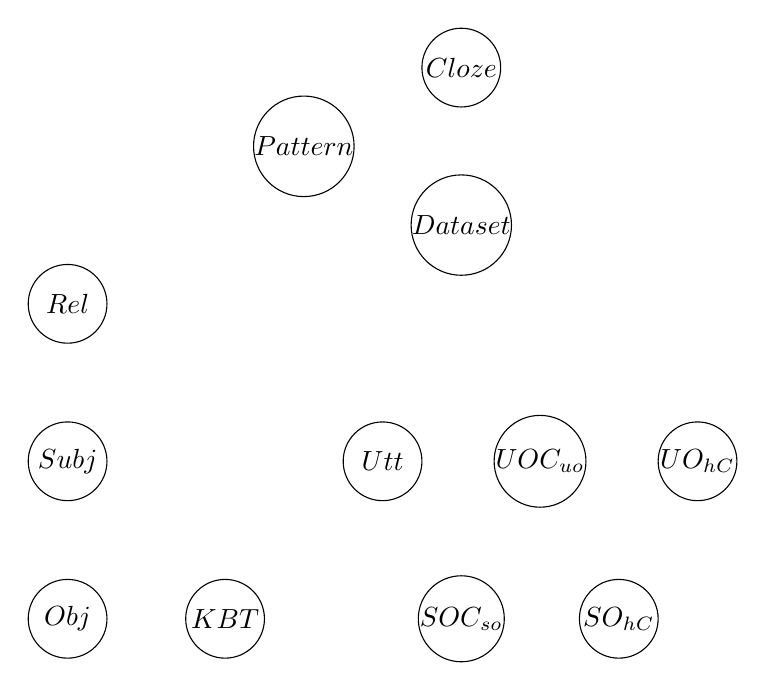
\begin{tikzpicture}[
  emb/.style={rectangle,draw,fill=white,minimum width=2cm,minimum height=0.6cm,rounded corners=.8ex},
  normal/.style={rectangle,draw,fill=white,minimum width=4cm,minimum height=0.8cm,rounded corners=.8ex},
  path_embedding/.style={rectangle,draw,fill=blue!20,minimum width=4cm,    minimum height=0.7cm},
  nc_embedding/.style={rectangle,draw,fill=orange!50,minimum width=2.5cm,    minimum height=0.7cm},
  word_embedding/.style={rectangle,draw,fill=my_green!40,minimum width=2.5cm,    minimum height=0.7cm},
  every neuron/.style={circle,draw,fill=orange!50,minimum size=0.5cm},
  every neuron1/.style={circle,draw,fill=orange!50,minimum size=0.5cm},
  every neuron2/.style={circle,draw,fill=blue!50,minimum size=0.5cm},
  every neuron3/.style={circle,draw,fill=green!50,minimum size=0.5cm},
  every neuron4/.style={circle,draw,fill=cyan!50,minimum size=0.5cm},
  every neurontar/.style={circle,draw,fill=brown!50,minimum size=0.5cm},
  every text-box/.style={rectangle,minimum size=0.6cm},
  every rect/.style={rectangle,draw,fill=gray!50,minimum size=0.6cm},
  every rect0/.style={rectangle,draw,fill=gray!50,minimum size=0.6,opacity=0},
  every vecrec/.style={rectangle,draw,fill=none,minimum width=1.5cm, minimum height=0.8cm},
  every oper/.style={rectangle,draw,fill=yellow!50,minimum size=0.5cm},
  every oper1/.style={rectangle,draw,fill=red!50,minimum size=0.5cm},
  every oper2/.style={rectangle,draw,fill=pink!50,minimum size=0.5cm},
  neuron missing/.style={draw=none,fill=none,scale=2,execute at begin node=\color{black}$\cdots$}
  ]
  
  	

    
%\node [every neuron/.try, neuron 1/.try] (wemb-00) [] {};

\node[draw,circle,minimum size=1cm,inner sep=0pt] at (0,0) {$Rel$};
\node[draw,circle,minimum size=1cm,inner sep=0pt] at (0,-2) {$Subj$};
\node[draw,circle,minimum size=1cm,inner sep=0pt] at (0,-4) {$Obj$};
\node[draw,circle,minimum size=1cm,inner sep=0pt] at (2,-4) {$KBT$};


\node[draw,circle,minimum size=1cm,inner sep=0pt] at (5,-4) {$SOC_{so}$};
\node[draw,circle,minimum size=1cm,inner sep=0pt] at (7,-4) {$SO_{hC}$};

\node[draw,circle,minimum size=1cm,inner sep=0pt] at (4,-2) {$Utt$};
\node[draw,circle,minimum size=1cm,inner sep=0pt] at (6,-2) {$UOC_{uo}$};
\node[draw,circle,minimum size=1cm,inner sep=0pt] at (8,-2) {$UO_{hC}$};


\node[draw,circle,minimum size=1cm,inner sep=0pt] at (3,2) {$Pattern$};

\node[draw,circle,minimum size=1cm,inner sep=0pt] at (5,3) {$Cloze$};
\node[draw,circle,minimum size=1cm,inner sep=0pt] at (5,1) {$Dataset$};



    % textual explanation
    
%    \node [every text-box/.try, text-box 1/.try, text width=3.5cm,align=center] (transformer) [above right=1.7 and 8.25 of Middle-emb-0] {\textbf{Transformer}};
    

    

    
\end{tikzpicture}

\end{document}